%!TEX root = ResearchPlan_v2.tex
\section{Research methods and material, support from research environment} %%%%%%%%%%%%%%%%%%%%%%%%%%%%%%%%%%%%%%%%%%
%%%%%
\label{sec:researchmethods}

\textcolor{blue}{1st DRAFT VERSION}

The field of heavy ion physics has very vivid cross talk between theoreticians and experimentalist world wide. This is seen, for example, in the development of the analysis methods~\cite{Poskanzer:1998yz,Bilandzic:2010jr}, detailed phenomenological modeling such that underlying theories are compared with the data~\cite{Burke:2013yra,Renk:2011gj,Niemi:2015qia} and tuning and development of the heavy ion event generators~\cite{Gyulassy:1994ew,Lin:2004en,Lokhtin2006}. For example, in the flow analysis, this interplay has been realized in the correlations between flow harmonics~\cite{Poskanzer:1998yz,ALICE:2011ab} and event plane angles~\cite{Aad:2014fla,Bhalerao:2014xra} that are crucial starting points in this application. Two particle correlations have been a long established tool in heavy ion physics~\cite{PhysRevLett.95.152301,PhysRevLett.97.052301} and this line is currently developing to various jet-hadron correlation, see e.g.~\cite{Khachatryan:2016tfj}. 

Observing the Mach cone in heavy ion collisions, or studying hard-soft interactions in general, has been a goal for a long time. After the observed cone-line structure in azimuthal correlations turned out be explained by the collective flow~\cite{ALICE:2011ab} and more detailed study of distribution of the hard interaction vertices was found out to smear the signal~\cite{Tachibana:2015qxa}, it is clear this proposal possesses a risk the positive observation may not come. However, the development in the field is astonishing, taking for example the correlations of the flow coefficients now measure correlations strengths that are order of part per million over the average values~\cite{ALICE:2016kpq} and the phenomena have a valid theoretical description. Heavy ion physics is clearly entering to the precision measurements where large statistics measurements enable extraction of weaker signals. Also, the steps towards the goal will provide results that are very valuable in discriminating and refining the current phenomenological models.

The research tools and methods are state of the art and under significant international interest and development. Our group has significant experience on output from flow, jet and correlation analysis methods, as will be summarized in~\label{sec:reseachteam}, so we have the neccessary qualifications to this project.

Obviously CERN is one of the best environments in the whole world to carry out this research. In ALICE experiment, the physics analyses are performed in the Physics Working Groups (PWG) that collect world wide researchers that are interest in a particular topic. Our group is involved in PWG's for correlation and flow analysis, and a PWG for jet analysis. The analysis work is supported and steered by the PWG's and a good interaction in the group provides a constant feedback and steady path to publish the results.

Department of Physics in Jyv\"askyl\"a has a long tradition in heavy ion physics dating back to early works by Vesa Ruuskanen and his collaborations \cite{VonGersdorff:1986tqh}. The experimental involvement started heavily when Jyv\"askyl\"a and HIP committed themselves to design and build the T0 timing detector to ALICE and production SSD modules to ALICE inner tracker~\cite{Dellacasa:1999kf}. Currently particle physics, and ultra-relativistic heavy ion collisions, is one of the main research lines in Jyv\"askyl\"a to which the department is fully committed itself. In wider perspective, it is also part of the "Structure of Matter with Accelerator Methods" to which Academy of Finland has granted profiling funding to University of Jyv\"askyl\"a. In theory side we have a strong group lead by Academy project leader and professor Kari Eskola and ERC Consolidator grant holder Tuomas Lappi, both internationally recognized experts in the heavy ion physics. Our group governs the Finnish participation to ALICE experiment trough a project in Nuclear Matter program in HIP. Together with the local cosmology and neutrino physics group, the department has build an extensive teaching program in various topics in particle physics up to a high level post graduate courses both in experimental and theoretical side. We have a common seminar with the theory group and untrammeled interaction between the groups.

Research results in this project come from analyzing the data with self-written codes. In following I will provide a brief description on how the data management goes in practice.  The raw data for this project (order of 10 petabytes of raw data every calendar year) will be collected by the ALICE experiment at CERN. Preservation and availability of this data is under the CERN's own data management plan and taken care of internationally.

All data measured by the ALICE experiment are available in LHC grid. Team of professionals will mine the raw detector data into more user friendly analysis files (Analysis Object Data (AOD)), where one has physical objects, like charged tracks or calorimeter clusters, from all good runs and events in some data taking periods. These files are stored, backed up and made available by CERN. Every research team in the collaboration can participate into Quality Assurance of the data and AOD's are updated by the findings of the analyzers.

In practice that data analysis has following guidelines: All the analysis code is written to so called AliRoot\footnote{http://aliroot-docs.web.cern.ch/aliroot-docs/} code packet, which is a GIT-repository (version control system) governed by CERN. Every analyzer belongs into some Physics Working Group (PWG) under which she develops her own analysis code. All the analysis code is first tested locally and then committed into this experiment wide GIT-repository, assuming that it passes quality criteria set by the experiment. By the latest at this point, the code that analyzer produced is stored and backed up with full version control. 

In ALICE, the data is recommended to be mined in so called ``lego train framework'' \cite{Zimmermann:2015owa}. This means that the analysis code that is committed into AliRoot will run over the desired data sets in the LHC grid environment semi-automatically and user can collect the ready analysis results from the data mining from grid to his local computer.

In the final state, analyzer develops an analysis and Figure plotting macro locally to reach the very final analysis results. These results are first approved by the PWG and later exposed to the whole collaboration to get the ALICE preliminary status. All analysis must be accompanied with very detailed internal analysis note. This note together with all analysis and figure plotting macros are stored in the internal pages of the ALICE experiment and hence all the documentation and all the final codes are fully stored, backed up with version control and made available to the collaboration. LHC experiments prepare also public analysis notes where certain analysis details, that will not come out along papers, are made publicly available. CERN has committed itself to fully open access publishing of all the scientific results obtained at CERN.

\section{Ethical issues}

There is no need of ethical considerations in any of the research done in ALICE experiment at the Large Hadron Collider in CERN.


\section{Implementation: schedule, budget, distribution of work} %%%%%%%%%%%%%%%%%%%%%%%%%%%%%%%
\label{sec:implementation}

\textcolor{blue}{NOT AT ALL FINISHED.}

Figure~\ref{fig:LHC-mid-term} shows the medium term running plan of the LHC. 
%%%%%%%%%% BEGIN FIGURE %%%%%%%%%%%%%%%%
\begin{figure}[htbp]
   \centering
   \resizebox{15cm}{!}{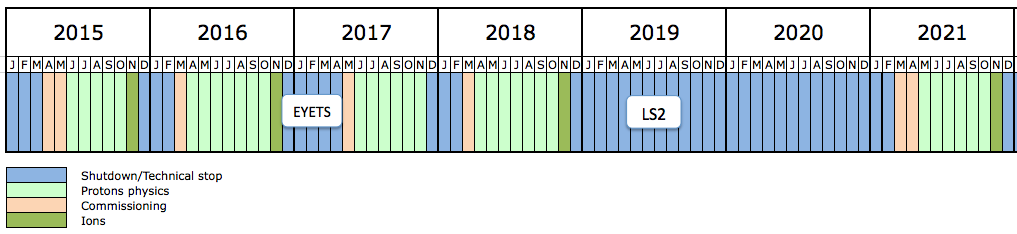
\includegraphics{LHC-medium-term.png}}
   \caption{Current draft of the medium term LHC running plan.}
   \label{fig:LHC-mid-term}
\end{figure}
%%%%%%%%%% END FIGURE %%%%%%%%%%%%%%%%%
The LHC experiments measured lead-lead data in 2015 and proton-lead at the end of 2016. Both campaigns went well and LHC performed very well. Due to Extended Year End Technical Stop (EYETS) at the end of 2017, aiming to reduce workload that LHC would otherwise face during the Long Shutdown 2 (LS2), there won't be heavy ion beam(s) at the LHC in 2017. However, one more lead-lead campaign will take place at the end of Run2 in December 2018, before the LS2 starts.

Year 2010 and 2011 heavy ion data (Run1) was taken at lower energy, $\sNN=2.76$~TeV, and 2015 data (Run2) with higher energy, $\sNN=5.02$~TeV. As ALICE reached the nominal design luminosity in 2015, that data set has 100 times more statistics compared to 2011 data set, that already was larger than 2010. However, we also experienced tracking problem in TPC due to accumulated space charge in high luminosity runs. Due to that, calibration of 2015 data needed significantly more effort than earlier data sets, but now this high-luminosity data set \textcolor{blue}{starts to be / is??} ready to be anylysed. \textcolor{blue}{The lead-lead campaign at the end of 2018 will be with the same energy, $\sNN=5.02$~TeV.} EMCal jet trigger was operational in 2015 Pb+Pb data taking and 2018 running should also contain rare triggers. Assuming that calibration of the 2018 lead-lead data goes well in 2019, we will have very significant statistics available for the analysis in 2020.

%%%%%%%%%%%%%% TABLE : TimeTable for the analysis %%%%%%%%%%%
%\begin{table}[htdp]
\begin{table}[htp]
\caption{Rough timetable for expected milestones in the analysis.}
\begin{center}
\begin{tabular}{ L{1.6cm} | L{11.5cm} | L{1.0cm} }
Assigned & Task & Year \\
\hline
PhD-     & Finishing the analysis on higher harmonic flow correlation  & 2018\\
student & ALICE publication from higher harmonic flow correlation & 2019 \\
 Jasper   & Finalize PhD-thesis on higher harmonic flow correlation & 2021 \\
 Parkkila & PhD-studies (40 cr) and 6 months of Service Work (20 cr) &  \\
\hline
              & Jet - and di-jet events in 2015 lead-lead data  & 2019 \\
Post doc & Starting systematic studies on event section criteria of jets & 2019 \\
  N.N.     & Final paper for "Interplay of Hard and Soft Physics"  & 2021 \\
              & EMCal trigger commissioning &  2021 \\
              & EMCal trigger maintenance &  2022 \\
\hline
 Together& Soft-hard analysis: flow in events biased with presence of a hard (di-)jet & 2020 \\
\hline
\end{tabular}
\end{center}
\label{tab:timetable}
\end{table}
%%%%%%%%%%%%%% END TABLE %%% %%%%%%%%%%%

As the pre-requisites studies for correlations of flow harmonics from Run1 will be finalized in 2017, quite likely close to beginning of this application period, we will be in very good position to start the analysis outlined here. Table~\ref{tab:timetable} shows the outline we find realistic for studies that will combine current flow analysis to event selection bias coming from presence of hard jets.

One should note that the above is only for the analysis. Post doc will have to use fraction of his/her time for the EMCal trigger maintenance. PhD-student must give equivalent of total of 6 months of full working time to ALICE experiments service work. Regarding our obligations, the PhD student will be quite likely involved also in the TPC upgrade activities. The exact timing either to LS2 or preceding QA work will depend on the need. Our group members have to participate into our institutional share of the ALICE shift load during running of the experiment.

This applications has mainly salary and mobility allowances together with some travel costs which makes the budgeting in principle rather straightforward. We apply here a salary for a post doc and PhD-student positions, see Table~\ref{tab:money} for average yearly costs.
%%%%%%%%%%%%%% TABLE : MONEY %%%%%%%%%%%
\begin{table}[htp]
\caption{Main expenses in a yearly budget.}
\begin{center}
\begin{tabular}{l|l|r|r|r|r}
Position & Assignment & Salary & Mobility & Travel & Tot. cost\\
& & month & year & year & year \\\hline
Post doc & Analysis + EMCal running    & 3'350 & 12'600 & 2'000 & 116'762\\
PhD student & Analysis + TPC upgrade & 2'200 &  See text   & 2'000 & 69'090 \\
PI & Project leading & 6'000 &  See text   & See text & 22'870 \\
\multicolumn{5}{r}{Average full cost/year} & 208'722  \\
\end{tabular}
\end{center}
\label{tab:money}
\end{table}
%%%%%%%%%%%%%% END TABLE %%% %%%%%%%%%%%
As the post doc should be 100~\% of the time at CERN, due to planned responsibilities in EMCal running and maintenance, he/she would need (minimum) of $12\times1050$~\euro$/{\rm m}=12600$~\euro\ per year the mobility money. Also the PhD-student needs to spend significant time in CERN to perform the service work duties, do shifts and interact with Physics Working Group. Due to project size limitations, we could not embed his/her mobility costs to this application. We will use some other source, like annual HIP ALICE project resources, to this purpose.

Currently the post doc is not named, so this position would go into international call. Quite likely a suitable candidate could be a recently defended PhD inside the ALICE experiment, who has background in flow or EMCal jet analysis. He/she would then be very familiar with the experiment and analysis environment. Our group has a very good candidate to the PhD-student position, Jasper Parkkila. Jasper worked in our group in HIP's summer student program in 2016 and made very impressive student work when he participated to flow analysis that is going to published. Jasper is expected to finish his Master's Thesis in May-August 2017 so this project would provide him a secure funding for his PhD-thesis.

I would meet and supervise both post doc and PhD-student in CERN personally, as I spend a significant portion of the calendar year there all the time. In typical calendar year I am on-site at CERN roughly 6 months. I am also Finnish representative in ALICE collaboration board that requires presense at CERN, on top of the leading this project. Since I have also other duties on-site at CERN, my mobility expenses are covered by the direct funding that Ministry of Education provides to Finnish ALICE activities.

Also two senior members of the group, DongJo Kim and Sami R\"as\"anen, visit in CERN regularly and support the work of both. DongJo is a flow expert in our group and would be the co-supervisor in the PhD-students thesis work. Sami has a background in theory accompanied with significant teaching and student councelling experience, so he will make a contribution to steering of the analysis and how the results are related with theoretical studies.


\nopagebreak
